\chapter{Research Problem} \label{chap:problem}

This chapter intends to clarify the problem addressed by the present dissertation. 

\section{Problem Statement} \label{sec:prob-state}

As previously mentioned in chapter \ref{chap:intro}, it is considered a scenario where an AUV is taking part on a long-term underwater mission. When it is in course, the moving survey AUV periodically sends known signals to the surface with a pinger, so it can be identified. The mule AUV, which is provided with a three dimensional array of hydrophones, receives the signal and estimates the position of the other AUV to navigate near it. The described communication system is illustrated in figure \ref{fig:auv_scene}. 

\note{redefinir}

\begin{figure}[!htbp]
	\centering
	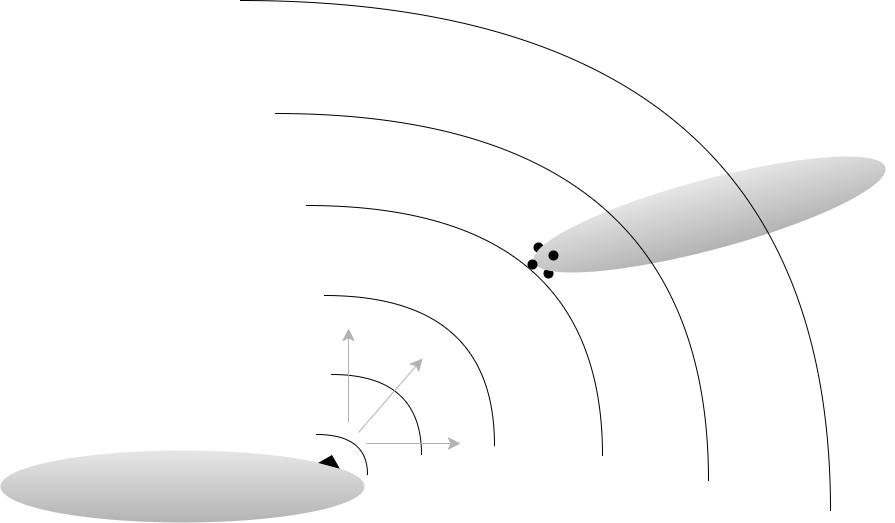
\includegraphics[width=0.7\textwidth]{figures/proposed-solution}
	\caption{Communication System}
	\label{fig:auv_scene}
\end{figure}

This partial system was developed in previous dissertations and research work, which can be better understood in \cite{afonso-thesis}. Briefly, the system consists on a transducer of four hydrophones forming a 3D array deployed on the mule AUV. This array will receive the same signal wave front. The system then calculates the cross-correlation between the received and expected signals, which is a BPSK modulated binary sequence. The cross-correlation peak indicates the distance between AUVs and it is calculated with timing resolution corresponding to 1 sampling period of the acquired signal, which in the developed systems corresponds approximately to 6mm (with a sampling frequency of 244kHz).

Since we are referring to an USBL system and due to the limitations in dimension of the AUV that will integrate this system, the hydrophones have to be placed within a few centimeters from each other. For this reason, the obtained time resolution by using only the cross-correlation, corresponding to a maximum distance accuracy of approximately 6mm, will not be enough for the calculation of the angle of arrival of the sound wave. Thus, in this thesis it is intended to refine this measurement by additionally calculating the phase differences of the arriving signals to each hydrophone. 

Upon having this measurement refined, the information of the phase difference between hydrophones, as well as additional data from modules already implemented, will serve as base to develop a software mechanism that estimates the angle of arrival of the received signal to the hydrophone array.

Finally, as an effort to improve the underwater localization system, a set of tests have to be performed in order to evaluate the robustness and estimation accuracy of the developed system. This study intends to prove the hypothesis declared in \ref{sec:hypoth-rq} and consequently respond to some of the defined research questions.


\section{Hypothesis and Research Questions} \label{sec:hypoth-rq}

This dissertation intends to complement previous research work by adding the design of an integral hardware model and respond to a core research hypothesis which serves as fundamental investigation purpose.

The first part of the developed work focuses on the practical implementation of a HDL model which has as premise the following idea: \textit{"Implementing a system that utilizes the phase differences between the arriving signals to an array of hydrophones, increases the accuracy of the time of arrival determination of the current system, which consequently improves the angle of arrival estimation."}

The second part of the research work focuses on the study and experimentation with methods that improve the localization accuracy for underwater applications. This research hypothesis can be stated as:
\\

\textit{"Using a real-time dynamic reconfigurable hydrophone array improves the underwater localization accuracy"}
\\

Attending the proposed hypothesis, the topics that are intended to be explored and discussed in this thesis's work can be summarized in the following research questions:

%Research Questions
\begin{itemize}

	\item \textbf{RQ1: }\textit{How should a system be implemented so it is capable of calculating phase differences between arriving signals at four different hydrophones and, simultaneously, be compatible with the available space in the FPGA?}
	
	\item \textbf{RQ2: }\textit{What method should be adopted in order to efficiently estimate the angle of arrival of a signal to an array of four hydrophones?}
	
	\item \textbf{RQ3: }\textit{What metrics should be used to evaluate which hydrophone configuration is optimal for a certain angle of arrival?}
	
	\item \textbf{RQ4: }\textit{How should the system be developed in order to improve the vision angle of the hydrophone array?}
	
\end{itemize}

These questions summarize the main topic points which are explored in the scope of this thesis and are the essential inquiries that it intends to answer.


\section{Validation Methods} \label{sec:validation}

The validation of scientific work is a key factor to demonstrate how reliable and effective it is. In this thesis, three essential methods are used to validate the functionality of the developed techniques:

\begin{itemize}
	
	\item \textbf{Simulation}
	
	The considered immediate approach to evaluate the functionality and behavior of the system consists in creating a set of simulation procedures which are as close as possible to the real environment and the physical system. These simulations were made as MATLAB scripts carefully designed to integrate realistic parameters, such as expected environment noise and other limitations.
	
	\item \textbf{Scientifically recognized methods}
	
	When composing a system, it can be useful comparing the studied approach with widely used methods which are recognized in the scientific community as robust and trustworthy. By doing this, we can gain a level of confidence in the developed system and in the obtained results.
	
	\item \textbf{Field experiments}
	
	After having the analytical methods and simulations coherent, it is essential then to test the system in a real environment in order to understand if the system still works correctly when real conditions are added. By testing it in a real application it is possible to take conclusions about its robustness and consider improvements or refinements for the system.
	
\end{itemize}
